\documentclass{article}

\usepackage[utf8]{inputenc}
\usepackage[english]{babel}
\usepackage{cite}
\usepackage{nameref,hyperref}
\usepackage[right]{lineno}
\usepackage{multirow}
\usepackage{adjustbox}
\usepackage[toc,page]{appendix}
\usepackage[table]{xcolor} 
\usepackage{pbox}

\bibliographystyle{../bibliography/plos2015}

% \setkeys{Gin}{width=1.2\textwidth}

\makeatletter
\renewcommand{\@biblabel}[1]{\quad#1.}
\makeatother

\providecommand{\keywords}[1]{\textbf{\textit{Keywords:}} #1}

% Leave date blank
% \date{}

\title{Too good to be false: Nonsignificant results revisited}
\author{CHJ Hartgerink\textsuperscript{1}, JM Wicherts\textsuperscript{1}, MALM van Assen\textsuperscript{1}\\ \\
\textsuperscript{1}Tilburg University, the Netherlands}

\usepackage{Sweave}
\begin{document}
\Sconcordance{concordance:manuscript.tex:manuscript.Rnw:%
1 30 1 1 0 13 1 1 30 101 1 1 25 1 34 1 69 5 1 1 16 33 1 1 66 22 1 1 212 %
14 1 1 182 83 1 1 46 53 1 1 159 71 1}

\maketitle

\begin{abstract}
Due to its probabilistic nature, Null Hypothesis Significance Testing (NHST) is subject to decision errors. The concern for false positives has overshadowed the concern for false negatives in the recent debates in psychology, which seems unwarranted. Our study demonstrates the importance of paying attention to false negatives alongside those significant results that may be 'too good to be true'; nonsignificant results may be 'too good to be false'. We examined evidence for false negatives in nonsignificant results in three different ways. To this end, we adapted the Fisher method to detect the presence of at least one false negative in a set of statistically nonsignificant results; simulations indicated it to be a powerful method for that purpose. The three applications indicated that (i) approximately two out of three (66.7\%) psychology articles reporting nonsignificant results contain evidence for at least one false negative, (ii) nonsignificant results on gender effects contain evidence of true nonzero effects, and (iii) the statistically nonsignificant replications from the Reproducibility Project Psychology (RPP) do not warrant conclusions about the absence or presence of true zero effects underlying these nonsignificant results. False negatives deserve more attention in the debate among psychologists, because there is sufficient evidence in these three applications to indicate that false negatives are a threat to the scientific discovery process; it can be considered a waste of resources if effects are studied but results are neglected due to the lack of statistical power.
\end{abstract}

\keywords{nonsignificant, underpowered, effect size, Fisher test}

\section*{Author note}
All research files, data, and analyses scripts are preserved and made available for download at \url{http://doi.org/10.5281/zenodo.154514}.
\newpage


Popper's \cite{Popper2005-xu} falsifiability serves as one of the main demarcating criteria in the social sciences, which stipulates that a hypothesis is required to have the possibility of being proven false to be considered scientific. Within the theoretical framework of scientific hypothesis testing, accepting or rejecting a hypothesis is unequivocal, because the hypothesis is either true or false. Statistical hypothesis testing, on the other hand, is a probabilistic operationalization of scientific hypothesis testing \cite{meehl1978theoretical} and, in lieu of its probabilistic nature, is subject to decision errors. Such decision errors are the topic of this paper.

Null Hypothesis Significance Testing (NHST) is the most prevalent paradigm for statistical hypothesis testing in the social sciences \cite{American_Psychological_Association2010-qe}. In NHST the hypothesis $H_0$ is tested, where $H_0$ most often regards the absence of an effect. If deemed false, an alternative, mutually exclusive hypothesis $H_1$ is accepted. These decisions are based on the $p$-value; the probability of the sample data, or more extreme data, given $H_0$ is true. If the $p$-value is smaller than the decision criterion (i.e., $\alpha$; typically .05 \cite{Nuijten2015-od}), $H_0$ is rejected and $H_1$ is accepted.

Table \ref{tab:tab1} summarizes the four possible situations that can occur in NHST. The columns indicate which hypothesis is true in the population and the rows indicate what is decided based on the sample data. When there is discordance between the true- and decided hypothesis, a decision error is made. More specifically, when $H_0$ is true in the population, but $H_1$ is accepted ('$H_1$'), a Type I error is made ($\alpha$); a false positive (lower left cell). When $H_1$ is true in the population and $H_0$ is accepted ('$H_0$'), a Type II error is made ($\beta$); a false negative (upper right cell). However, when the null hypothesis is true in the population and $H_0$ is accepted ('$H_0$'), this is a true negative (upper left cell; $1-\alpha$). The true negative rate is also called specificity of the test. Conversely, when the alternative hypothesis is true in the population and $H_1$ is accepted ('$H_1$'), this is a true positive (lower right cell). The probability of finding a statistically significant result if $H_1$ is true is the power ($1-\beta$), which is also called the sensitivity of the test. Power is a positive function of the (true) population effect size, the sample size, and the alpha of the study, such that higher power can always be achieved by altering either the sample size or the alpha level \cite{Aberson2010-xa}. 

\begin{table}[htbp]
% \rowcolors{2}{gray!25}{white}
\caption{Summary table of possible NHST results. Columns indicate the true situation in the population, rows indicate the decision based on a statistical test. The true positive probability is also called power and sensitivity, whereas the true negative rate is also called specificity.}
\begin{adjustbox}{width=\textwidth,totalheight=\textheight,keepaspectratio,angle=0}
\centering
\begin{tabular}{llll}
&    & Population                        &                                    \\ \hline
&    & $H_0$                                & $H_1$                                 \\
Decision & '$H_0$' & $1-\alpha$                           & $\beta$                               \\
&    & True negative                     & False negative {[}Type II error{]} \\
& '$H_1$' & $\alpha$                             & $1-\beta$                             \\
&    & False positive {[}Type I error{]} & True positive                   \\  \hline
\end{tabular}
\end{adjustbox}
\label{tab:tab1}
\end{table}

Recent debate about false positives has received much attention in science and psychological science in particular. The Reproducibility Project Psychology (RPP), which replicated 100 effects reported in prominent psychology journals in 2008, found that only 36\% of these effects were statistically significant in the replication \cite{Open_Science_Collaboration2015-zs}. Besides psychology, reproducibility problems have also been indicated in economics \cite{Camerer2016-zz} and medicine \cite{Begley2012-uc}. Although these studies suggest substantial evidence of false positives in these fields, replications show considerable variability in resulting effect size estimates \cite{Klein2014-jb, Stanley2014-pd}. Therefore caution is warranted when wishing to draw conclusions on the presence of an effect in individual studies (original or replication; \cite{Open_Science_Collaboration2015-zs,Gilbert2016-mi,Anderson2016-bv}).

The debate about false positives is driven by the current overemphasis on statistical significance of research results \cite{Giner-Sorolla2012-wn}. This overemphasis is substantiated by the finding that >90\% of results in the psychology literature are statistically significant \cite{Open_Science_Collaboration2015-zs,Sterling1995-fe,Sterling1959-pf} despite low statistical power due to small sample sizes \cite{Cohen1962-jc,Sedlmeier1989-yc,Marszalek2011-rf,Bakker2012-tf}. Consequently, publications have become biased by overrepresenting statistically significant results \cite{Greenwald1975-ck}, which generally results in effect size overestimation in individual studies \cite{Nuijten2015-od} and in meta-analyses \cite{Van_Assen2015-gg,Lane_1978,Rothstein2005-zg,Borenstein2009-vs}. The overemphasis on statistically significant effects has been accompanied by questionable research practices (QRPs, \cite{John2012-uj}) such as erroneously rounding p-values towards significance, which for example occurred for 13.8\% of all $p$-values reported as "$p =.05$" in articles from eight major psychology journals in the period 1985-2013 \cite{Hartgerink2016-mm}.

The concern for false positives has overshadowed the concern for false negatives in the recent debate, which seems unwarranted. Cohen \cite{Cohen1962-jc} was the first to indicate that psychological science was (severely) underpowered, which is defined as the chance of finding a statistically significant effect in the sample lower than 50\% when there is truly an effect in the population. This has not changed throughout the subsequent fifty years \cite{Bakker2012-tf,Fraley2014-xs}. Given that the complement of true positives (i.e., power) are false negatives, no evidence either exists that the problem of false negatives has been resolved in psychology. Moreover, Fiedler, Kutzner, and Krueger \cite{Fiedler2012-gx} worry that an increased focus on false positives is too shortsighted, arguing that false negatives are more difficult to detect than false positives. They also argue that, because of the focus on statistically significant results, negative results are less likely to be the subject of replications than positive results, decreasing the probability of detecting a false negative. Additionally, the Positive Predictive Value (PPV; the number of statistically significant effects that are true \cite{Ioannidis2005-am}) has been a major point of discussion in recent years, whereas the Negative Predictive Value (NPV) is rarely mentioned.

The research objective of the current paper is to examine evidence for false negative results in the published psychology literature. To this end, we inspected a large number of nonsignificant results from eight flagship psychology journals. First, we compared the observed effect distributions of nonsignificant results for eight journals (combined and separately) to the expected null distribution based on simulations, where a discrepancy between observed and expected distribution was anticipated (i.e., presence of false negatives). Second, we propose to use the Fisher test to test the hypothesis that $H_0$ is true for all nonsignificant results reported in a paper, which we show to have high power to detect false negatives in a simulation study. Third, we applied the Fisher test to the nonsignificant results in 14,765 psychology papers from these eight flagship psychology journals to inspect how many papers show evidence of at least one false negative result. Fourth, we examined evidence of false negatives in reported gender effects. Gender effects are particularly interesting, because gender is typically a control variable and not the primary focus of studies. Hence we expect little $p$-hacking and substantial evidence of false negatives in reported gender effects in psychology. Finally, as another application, we applied the Fisher test to the 64 nonsignificant replication results of the RPP \cite{Open_Science_Collaboration2015-zs} to examine whether at least one of these nonsignificant results may actually be a false negative. 

\section*{Theoretical framework}

We begin by reviewing the probability density function of both an individual $p$-value and a set of independent $p$-values as a function of population effect size. Subsequently, we propose  a method to test whether a collection of nonsignificant results across papers deviates from what would be expected under the $H_0$. We also propose a method to test whether nonsignificant results deviate from $H_0$ within a paper. These methods will be used to test whether there is evidence for false negatives in the psychology literature.

\subsection*{Distributions of \textit{p}-values}

The distribution of one $p$-value is a function of the population effect, the observed effect and the precision of the estimate. When the population effect is zero, the probability distribution of one $p$-value is uniform. When there is a non-zero effect, the probability distribution is right-skewed. More specifically, as sample size or true effect size increases, the probability distribution of one $p$-value becomes increasingly right-skewed. These regularities also generalize to a set of independent $p$-values, which are uniformly distributed when there is no population effect and right-skew distributed when there is a population effect, with more right-skew as the population effect and/or precision increases \cite{Fisher1925-jl}.

Considering that the present paper focuses on false negatives, we primarily examine nonsignificant $p$-values and their distribution. Since the test we apply is based on nonselected $p$-values, it requires random variables distributed between 0 and 1. We apply the following transformation to each nonsignificant $p$-value that is selected
\begin{equation}
\label{pistar}
p^*_i=\frac{p_i-\alpha}{1-\alpha}
\end{equation}
where $p_i$ is the  reported nonsignificant $p$-value and $\alpha$ is the selected significance cutoff (i.e., $\alpha=.05$). Note this transformation retains the distributional properties of the original $p$-values for the selected nonsignificant results. Both one-tailed and two-tailed tests can be included in this way.

\subsection*{Testing for false negatives: the Fisher test}

We applied the Fisher test to inspect whether the distribution of observed nonsignificant $p$-values deviates from those expected under $H_0$. The Fisher test was initially introduced as a meta-analytic technique to synthesize results across studies \cite{Fisher1925-jl,Hedges1985-dy}. When applied to transformed nonsignificant $p$-values (see Equation \ref{pistar}) the Fisher test tests for evidence against $H_0$ in a set of nonsignificant $p$-values. In other words, the null hypothesis we test with the Fisher test is that all included nonsignificant results are true negatives. The Fisher test statistic is calculated as
\begin{equation}
\label{fishertest}
\chi^2_{2k}=-2\sum\limits^k_{i=1}ln(p^*_i)
\end{equation}
where $k$ is the number of nonsignificant $p$-values and $\chi^2$ has $2k$ degrees of freedom. A larger $\chi^2$ value indicates more evidence for at least one false negative in the set of $p$-values. We conclude that there is sufficient evidence of at least one false negative result, if the Fisher test is statistically significant at $\alpha=.10$, similar to tests of publication bias that also use $\alpha=.10$ \cite{Sterne2000-wh,Ioannidis2007-hh,Francis2012-kw}.

We estimated the power of detecting false negatives with the Fisher test as a function of sample size $N$, true correlation effect size $\eta$, and $k$ nonsignificant test results (procedure described in Appendix A). The three levels of sample size used in our simulation study (33, 62, 119) correspond to the  25th, 50th (median) and 75th percentiles of the degrees of freedom of reported $t$, $F$, and $r$ statistics in eight flagship psychology journals (see Application 1 below). Degrees of freedom of these statistics are directly related to sample size, for instance, for a two-group comparison including 100 people, df = 98. 

Table \ref{tab:tab2} summarizes the results for the simulations of the Fisher test when the nonsignificant $p$-values are generated by either small- or medium population effect sizes. Results for all 5,400 conditions can be found on the OSF (\url{osf.io/qpfnw}). The results indicate that the Fisher test is a powerful method to test for a false negative among nonsignificant results. For example, for small true effect sizes ($\eta=.1$), 25 nonsignificant results from medium samples result in 85\% power (7 nonsignificant results from large samples yield 83\% power). For medium true effects ($\eta=.25$), three nonsignificant results from small samples ($N=33$) already provide 89\% power for detecting a false negative with the Fisher test. For large effects ($\eta=.4$), 2 nonsignificant results from small samples already almost always detects all false negatives.

% IF YOU WANT TO RERUN SIMULATIONS, SEE CODE CHUNK "SIMULATIONS" IN APPLICATION 1
% Sorry, made this table manually so have to check manually with files data/N_33.csv etc.
\begin{table}[htbp]
\caption{Power of Fisher test to detect false negatives for small- and medium effect sizes (i.e., $\eta=.1$ and $\eta=.25$), for different sample sizes (i.e., $N$) and number of test results (i.e., $k$). Results of each condition are based on 10,000 iterations. Power was rounded to 1 whenever it was larger than .9995.}
\rowcolors{2}{gray!25}{white}
\begin{adjustbox}{width=\textwidth,totalheight=\textheight,keepaspectratio,angle=0}
\centering
\begin{tabular}{llllllll}
&        & $\eta=.1$ &         &        & $\eta=.25$ &         \\
& $N=33$ & $N=62$ & $N=119$ & $N=33$ & $N=62$ & $N=119$ \\
\hline
$k=1$ & 0.151 & 0.211 & 0.341 & 0.575 & 0.852 & 0.983 \\
$k=2$ & 0.175 & 0.267 & 0.459 & 0.779 & 0.978 & 1 \\
$k=3$ & 0.201 & 0.317 & 0.572 & 0.894 & 1 & 1 \\
$k=4$ & 0.208 & 0.352 & 0.659 & 0.948 & 1 & 1 \\
$k=5$ & 0.229 & 0.390 & 0.719 & 0.975 & 1 & 1 \\
$k=6$ & 0.251 & 0.434 & 0.784 & 0.990 & 1 & 1 \\
$k=7$ & 0.259 & 0.471 & 0.834 & 0.995 & 1 & 1 \\
$k=8$ & 0.280 & 0.514 & 0.871 & 0.998 & 1 & 1 \\
$k=9$ & 0.298 & 0.530 & 0.895 & 1 & 1 & 1 \\
$k=10$ & 0.304 & 0.570 & 0.918 & 1 & 1 & 1 \\
$k=15$ & 0.362 & 0.691 & 0.980 & 1 & 1 & 1 \\
$k=20$ & 0.429 & 0.780 & 0.996 & 1 & 1 & 1 \\
$k=25$ & 0.490 & 0.852 & 1 & 1 & 1 & 1 \\
$k=30$ & 0.531 & 0.894 & 1 & 1 & 1 & 1 \\
$k=35$ & 0.578 & 0.930 & 1 & 1 & 1 & 1 \\
$k=40$ & 0.621 & 0.953 & 1 & 1 & 1 & 1 \\
$k=45$ & 0.654 & 0.966 & 1 & 1 & 1 & 1 \\
$k=50$ & 0.686 & 0.976 & 1 & 1 & 1 & 1 \\

\hline
\end{tabular}
\end{adjustbox}
\label{tab:tab2}
\end{table}

\section*{Application 1: Evidence of false negatives in articles across eight major psychology journals}

To show that statistically nonsignificant results do not warrant the interpretation that there is truly no effect, we analyzed statistically nonsignificant results from eight major psychology journals. First, we investigate if and how much the distribution of reported nonsignificant effect sizes deviates from what the expected effect size distribution is if there is truly no effect (i.e., $H_0$). Second, we investigate how many research articles report nonsignificant results and how many of those show evidence for at least one false negative using the Fisher test \cite{Fisher1925-jl}.

\subsection*{Method}




APA style $t$, $r$, and $F$ test statistics were extracted from eight psychology journals with the \texttt{R} package \texttt{statcheck} \cite{Nuijten2015-od,Epskamp2015-ps}. APA style is defined as the format where the type of test statistic is reported, followed by the degrees of freedom (if applicable), the observed test value, and the $p$-value (e.g., $t(85)=2.86, p=.005$; \cite{American_Psychological_Association2010-qe}). The \texttt{statcheck} package also recalculates $p$-values. We reuse the data from Nuijten et al. (\url{osf.io/gdr4q};\cite{Nuijten2015-od}). Table \ref{tab:tab3} depicts the journals, the timeframe, and summaries of the results extracted. The database also includes $\chi^2$ results, which we did not use in our analyses because effect sizes based on these results are not readily mapped on the correlation scale. Two erroneously reported test statistics were eliminated, such that these did not confound results. 

The analyses reported in this paper use the recalculated $p$-values to eliminate potential errors in the reported $p$-values \cite{Bakker2011-hg,Nuijten2015-od}. However, our recalculated $p$-values assumed that all other test statistics (degrees of freedom, test values of $t$, $F$, or $r$) are correctly reported. These errors may have affected the results of our analyses. Since most $p$-values and corresponding test statistics were consistent in our dataset (90.7\%), we do not believe these typing errors substantially affected our results and conclusions based on them.

% Sorry, inserted table manually long time ago, need to check manually

% Insert table 3
\begin{table}[htbp]
\caption{Summary table of articles downloaded per journal, their mean number of results, and proportion of (non)significant results. Statistical significance was determined using $\alpha=.05$, two-tailed test}
\rowcolors{2}{gray!25}{white}
\begin{adjustbox}{width=\textwidth,totalheight=\textheight,keepaspectratio,angle=0}
\centering
\begin{tabular}{lrrrrr}
\pbox{3cm}{Journal (Acronym)}                                    & Time frame         & Results         & \pbox{1.5cm}{Mean results per article} & \pbox{1.5cm}{Significant (\%)}          & \pbox{2cm}{Nonsignificant (\%)}      \\
\hline
\pbox{3cm}{Developmental Psychology (DP)}                        & 1985-2013          & 30,920           & 13.5                    & \pbox{1.5cm}{24,584 (79.5\%)}           & \pbox{2cm}{6,336 (20.5\%)}           \\
\pbox{3cm}{Frontiers in Psychology (FP)}                         & 2010-2013          & 9,172            & 14.9                    & \pbox{1.5cm}{6,595 (71.9\%)}            & \pbox{2cm}{2,577 (28.1\%)}           \\
\pbox{3cm}{Journal of Applied Psychology (JAP)}                  & 1985-2013          & 11,240           & 9.1                     & \pbox{1.5cm}{8,455 (75.2\%)}            & \pbox{2cm}{2,785 (24.8\%)}           \\
\pbox{3cm}{Journal of Consulting and Clinical Psychology (JCCP)} & 1985-2013          & 20,083           & 9.8                     & \pbox{1.5cm}{15,672 (78.0\%)}           & \pbox{2cm}{4,411 (22.0\%)}           \\
\pbox{3cm}{Journal of Experimental Psychology: General (JEPG)}   & 1985-2013          & 17,283           & 22.4                    & \pbox{1.5cm}{12,706 (73.5\%)}           & \pbox{2cm}{4,577 (26.5\%)}           \\
\pbox{3cm}{Journal of Personality and Social Psychology (JPSP)}  & 1985-2013          & 91,791           & 22.5                    & \pbox{1.5cm}{69,836 (76.1\%)}           & \pbox{2cm}{21,955 (23.9\%)}          \\
\pbox{3cm}{Public Library of Science (PLOS)}                     & 2003-2013          & 28,561           & 13.2                    & \pbox{1.5cm}{19,696 (69.0\%)}           & \pbox{2cm}{8,865 (31.0\%)}           \\
\pbox{3cm}{Psychological Science (PS)}                           & 2003-2013          & 14,032           & 9                       & \pbox{1.5cm}{10,943 (78.0\%)}           & \pbox{2cm}{3,089 (22.0\%)}           \\
\hline
\textit{Totals}                                      & \textit{1985-2013} & \textit{223,082} & \textit{14.3}           & \pbox{1.5cm}{\textit{168,487 (75.5\%)}} & \pbox{2cm}{\textit{54,595 (24.5\%)}}\\
\hline
\end{tabular}
\end{adjustbox}
\label{tab:tab3}
\end{table}

First, we compared the observed nonsignificant effect size distribution (computed with observed test results) to the expected nonsignificant effect size distribution under $H_0$. The expected effect size distribution under $H_0$ was approximated using simulation. We first randomly drew an observed test result (with replacement) and subsequently drew a random nonsignificant $p$-value between 0.05 and 1 (i.e., under the distribution of the $H_0$). Based on the drawn $p$-value and the degrees of freedom of the drawn test result, we computed the accompanying test statistic and the corresponding effect size (for details on effect size computation see Appendix B). This procedure was repeated 163,785 times, which is three times the number of observed nonsignificant test results (54,595). The collection of simulated results approximates the expected effect size distribution under $H_0$, assuming independence of test results. We inspected this possible dependency with the intra-class correlation ($ICC$), where $ICC=1$ indicates full dependency and $ICC=0$ indicates full independence. For the set of observed results, the ICC for $p$-values was .001, indicating independence of $p$-values within a paper. The resulting, expected effect size distribution was compared to the observed effect size distribution (i) across all journals and (ii) per journal. To test for differences between the expected and observed nonsignificant effect size distributions we applied the Kolmogorov-Smirnov test. This is a non-parametric goodness-of-fit test for equality of distributions, which is based on the maximum absolute deviation between the independent distributions being compared (denoted $D$; \cite{Massey1951-gj}).

Second, we applied the Fisher test to test how many research papers show evidence of at least one false negative statistical result. To recapitulate, the Fisher test tests whether the distribution of observed nonsignificant $p$-values deviates from the uniform distribution expected under $H_0$. In order to compute the result of the Fisher test, we applied equations \ref{pistar} and \ref{fishertest} to the recalculated nonsignificant $p$-values in each paper ($\alpha=.05$).

\subsection*{Results}

\subsubsection*{Observed effect size distribution.}


Figure \ref{fig:fig1} shows the distribution of observed effect sizes (in $|\eta|$) across all articles and indicates that, of the 223,082 observed effects, 7\% were zero to small (i.e., $0\leq|\eta|<.1$), 23\% were small to medium (i.e., $.1\leq|\eta|<.25$), 27\% medium to large (i.e., $.25\leq|\eta|<.4$), and 42\% large or larger (i.e., $|\eta|\geq.4$; \cite{Cohen1988-wg}). This suggests that the majority of effects reported in psychology is medium or smaller (i.e., 30\%), which is somewhat in line with a previous study on effect distributions \cite{Gignac2016-je}. Of the full set of 223,082 test results, 54,595 (24.5\%) were nonsiginificant, which is the dataset for our main analyses. 

\begin{figure}
\begin{center}
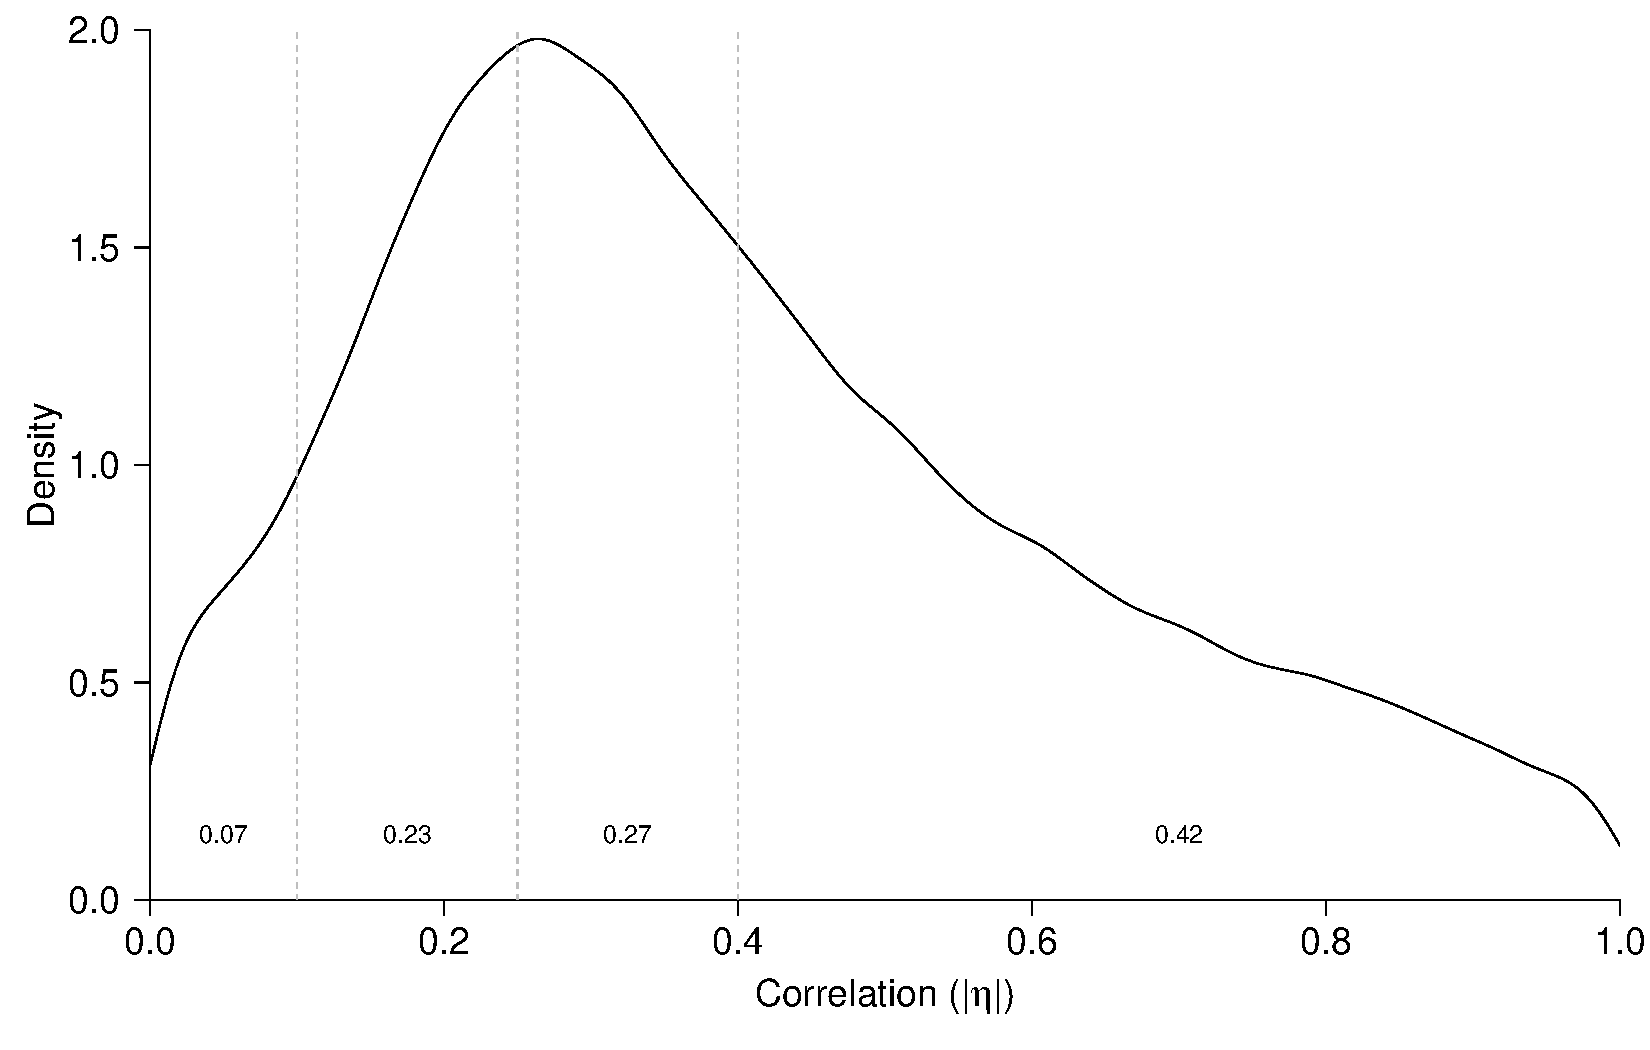
\includegraphics{../figures/Fig1.pdf}
\end{center}
\caption{Density of observed effect sizes of results reported in eight psychology journals, with 7\% of effects in the category none-small, 23\% small-medium, 27\% medium-large, and 42\% beyond large.}
\label{fig:fig1}
\end{figure}

Our dataset indicated that more nonsignificant results are reported throughout the years, strengthening the case for inspecting potential false negatives. The proportion of reported nonsignificant results showed an upward trend, as depicted in Figure \ref{fig:fig2}, from approximately 20\% in the eighties to approximately 30\% of all reported APA results in 2015.

\begin{figure}
\begin{center}
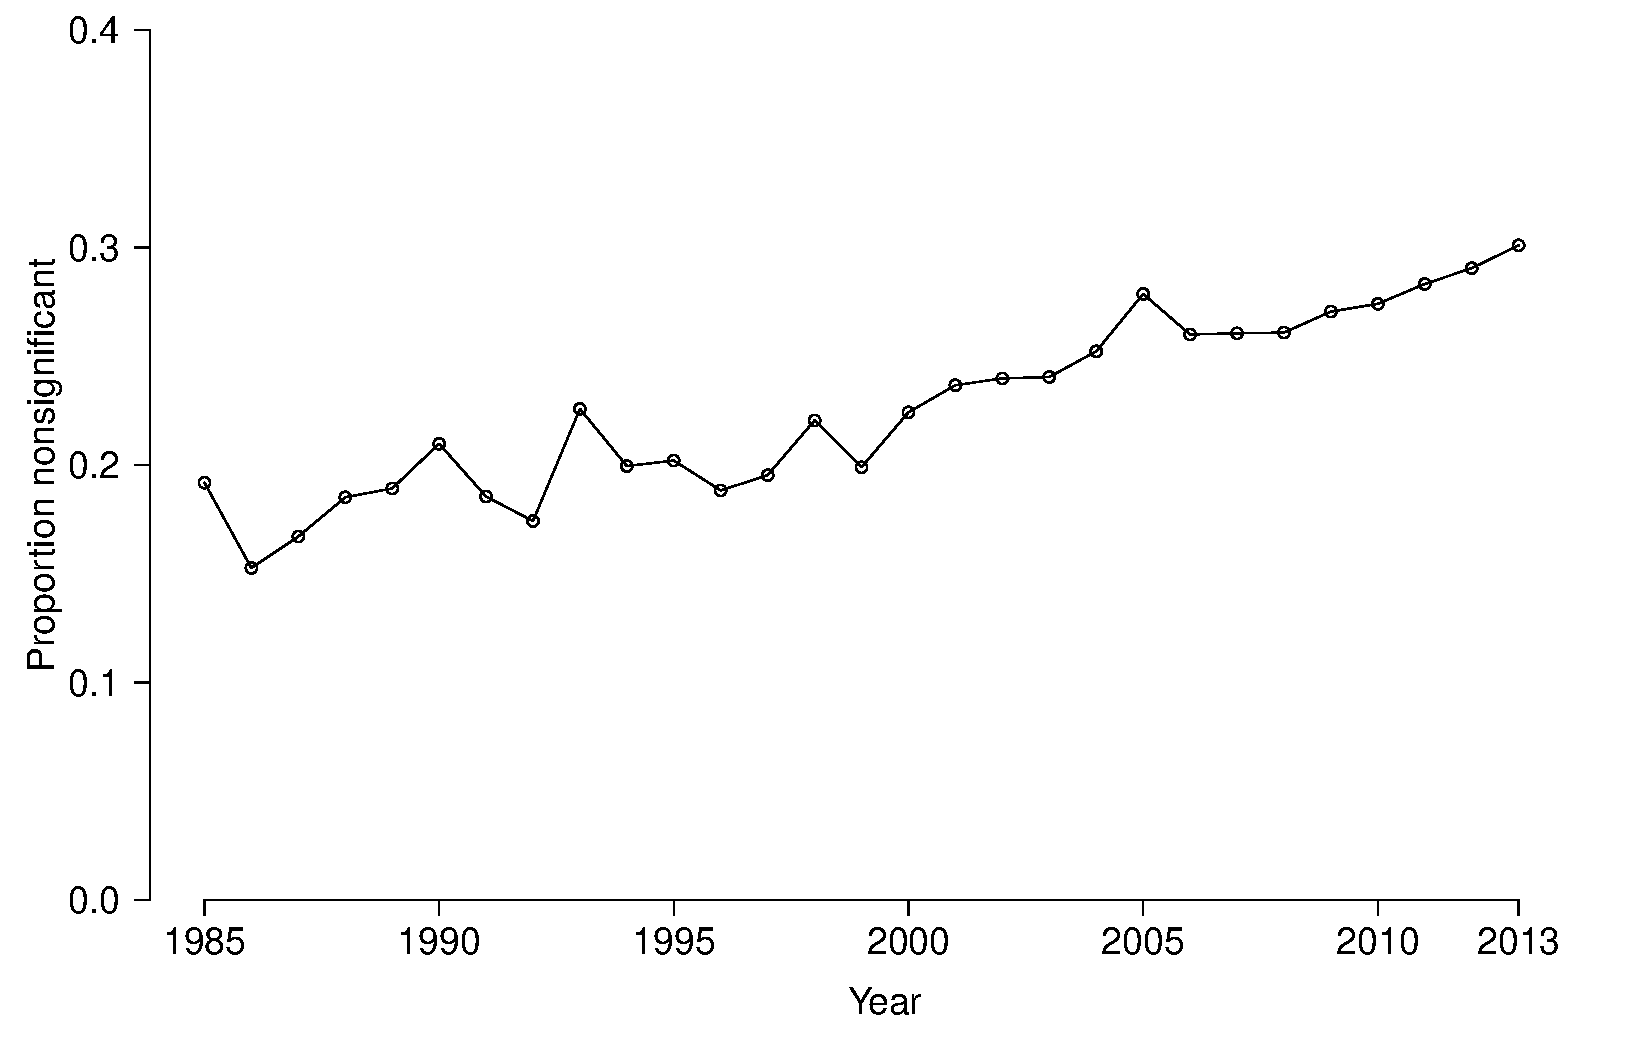
\includegraphics{../figures/Fig2.pdf}
\end{center}
\caption{Observed proportion of nonsignificant test results per year.}
\label{fig:fig2}
\end{figure}

\subsubsection*{Expected effect size distribution.}


For the entire set of nonsignificant results across journals, Figure \ref{fig:fig3} indicates that there is substantial evidence of false negatives. Under $H_0$, 46\% of all observed effects is expected to be within the range $0\leq|\eta|<.1$, as can be seen in the left panel of Figure \ref{fig:fig3} highlighted by the lowest grey line (dashed). However, of the observed effects, only 26\% fall within this range, as highlighted by the lowest black line. Similarly, we would expect 85\% of all effect sizes to be within the range $0\leq|\eta|<.25$ (middle grey line), but we observed 14 percentage points less in this range (i.e., 71\%; middle black line); 96\% is expected for the range $0\leq|\eta|<.4$ (top grey line), but we observed 4 percentage points less (i.e., 92\%; top black line). These differences indicate that larger nonsignificant effects are reported in papers than expected under a null effect. This indicates the presence of false negatives, which is confirmed by the Kolmogorov-Smirnov test, $D=0.3$, $p<.000000000000001$. Results were similar when the nonsignificant effects were considered separately for the eight journals, although deviations were smaller for the Journal of Applied Psychology (see \href{../figures/S1Fig}{Figure S1} for results per journal).

\begin{figure}
\begin{center}
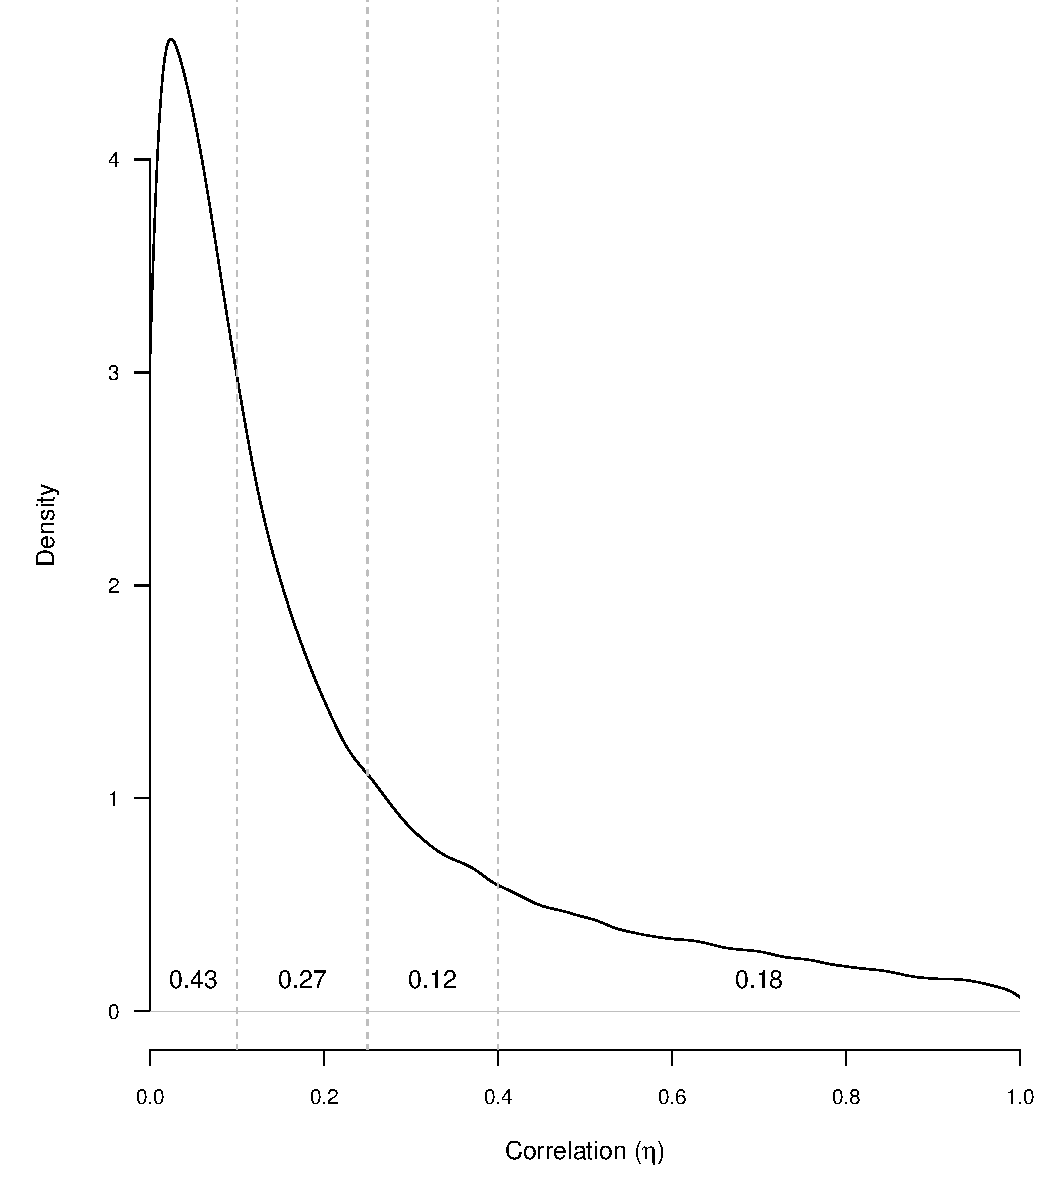
\includegraphics[width=\textwidth]{../figures/Fig3.pdf}
\end{center}
\caption{Observed and expected (adjusted and unadjusted) effect size distribution for statistically nonsignificant APA results reported in eight psychology journals. Grey lines depict expected values; black lines depict observed values. The three vertical dotted lines correspond to a small, medium, large effect, respectively. Header includes Kolmogorov-Smirnov test results.}
\label{fig:fig3}
\end{figure}

Because effect sizes and their distribution overestimate population effect size, particularly when sample size is small \cite{Voelkle2007-at,Hedges1981-og}, we also compared the observed and expected adjusted nonsignificant effect sizes that correct for such overestimation of effect sizes (right panel of Figure \ref{fig:fig3}; see Appendix B). The distribution of adjusted effect sizes of nonsignificant results tells the same story; observed effect sizes are larger than expected effect sizes. For instance, the distribution of adjusted reported effect size suggests 49\% of effect sizes are at least small, whereas under the $H_0$ only 22\% is expected.

\subsubsection*{Evidence of false negatives in articles.}


The Fisher test was applied to the nonsignificant test results of each of the 14,765 papers separately, to inspect for evidence of false negatives. More technically, we inspected whether $p$-values within a paper deviate from what can be expected under the $H_0$ (i.e., uniformity). If $H_0$ is in fact true, our results would be that there is evidence for false negatives in 10\% of the papers (a meta-false positive). Table \ref{tab:tab4} shows the number of papers with evidence for false negatives, specified per journal and per $k$ number of nonsignificant test results. The first row indicates the number of papers that report no nonsignificant results. Overall results (last row) indicate that 47.1\% of all articles show evidence of false negatives (i.e. 6,951 articles), and 66.7\% of articles reporting at least one result.

%Sorry, this table was manually done prior to Sweave. Manually check with code in above chunk
\begin{table}[htbp]
\caption{Summary table of Fisher test results applied to the nonsignificant results ($k$) of each article separately, overall and specified per journal. A significant Fisher test result is indicative of a false negative (FN). DP = Developmental Psychology; FP = Frontiers in Psychology; JAP = Journal of Applied Psychology; JCCP = Journal of Consulting and Clinical Psychology; JEPG = Journal of Experimental Psychology: General; JPSP = Journal of Personality and Social Psychology; PLOS = Public Library of Science; PS = Psychological Science.}
\rowcolors{2}{gray!25}{white}
\begin{adjustbox}{width=\textwidth,totalheight=\textheight,keepaspectratio,angle=0}
\centering
\begin{tabular}{lllllllllll}
 &  & Overall             & DP                & FP     & JAP    & JCCP   & JEPG   & JPSP   & PLOS   & PS \\
\hline
& Nr. of papers     & 14,765  & 2,283   & 614    & 1,239   & 2,039   & 772    & 4,087   & 2,166   & 1,565   \\
$k=0$               & Count             & 4,340   & 758    & 133    & 488    & 907    & 122    & 840    & 565    & 527    \\
& \%                & 29.4\% & 33.2\% & 21.7\% & 39.4\% & 44.5\% & 15.8\% & 20.6\% & 26.1\% & 33.7\% \\
\hline
$k=1$               & Evidence FN       & 57.7\% & 66.1\% & 41.2\% & 48.7\% & 58.7\% & 51.4\% & 66.0\% & 47.2\% & 56.4\% \\
& Count             & 2,510   & 433    & 102    & 238    & 380    & 109    & 556    & 339    & 353    \\
$k=2$               & Evidence FN       & 60.6\% & 66.9\% & 50.0\% & 36.3\% & 57.7\% & 66.7\% & 75.2\% & 51.6\% & 57.1\% \\
& Count             & 1,768   & 293    & 64     & 157    & 227    & 81     & 424    & 289    & 233    \\
$k=3$               & Evidence FN       & 65.3\% & 69.8\% & 57.6\% & 53.1\% & 54.4\% & 77.1\% & 80.6\% & 47.8\% & 60.2\% \\
& Count             & 1,257   & 199    & 66     & 98     & 125    & 83     & 341    & 184    & 161    \\
$k=4$               & Evidence FN       & 68.7\% & 75.0\% & 63.8\% & 53.1\% & 69.7\% & 67.9\% & 81.4\% & 52.7\% & 62.5\% \\
& Count             & 892    & 128    & 47     & 64     & 89     & 56     & 264    & 148    & 96     \\
$5\leq k<10$  & Evidence FN       & 72.3\% & 71.2\% & 67.7\% & 56.7\% & 66.3\% & 71.2\% & 87.1\% & 52.4\% & 63.0\% \\
& Count             & 2,394   & 326    & 124    & 134    & 208    & 163    & 898    & 368    & 173    \\
$10\leq k<20$ & Evidence FN       & 77.7\% & 76.9\% & 67.7\% & 60.0\% & 72.4\% & 81.2\% & 88.1\% & 57.3\% & 81.0\% \\
& Count             & 1,280   & 121    & 65     & 55     & 87     & 117    & 596    & 218    & 21     \\
$k\geq20$              & Evidence FN       & 84.0\% & 76.0\% & 53.8\% & 60.0\% & 87.5\% & 80.5\% & 94.0\% & 69.1\% & 0.0\%  \\
& Count             & 324    & 25     & 13     & 5      & 16     & 41     & 168    & 55     & 1      \\
\hline
All                 & Evidence FN       & 47.1\% & 46.5\% & 45.1\% & 29.9\% & 34.3\% & 59.1\% & 64.6\% & 38.4\% & 39.3\% \\
& Evidence FN $k\geq1$ & 66.7\% & 69.6\% & 57.6\% & 49.4\% & 61.7\% & 70.2\% & 81.3\% & 51.9\% & 59.2\% \\
& Count             & 6,951   & 1,061   & 277    & 371    & 699    & 456    & 2,641   & 831    & 615   \\
\hline
\end{tabular}
\end{adjustbox}
\label{tab:tab4}
\end{table}

Table \ref{tab:tab4} also shows evidence of false negatives for each of the eight journals. The lowest proportion of articles with evidence of at least one false negative was for the Journal of Applied Psychology (49.4\%; penultimate row). The remaining journals show higher proportions, with a maximum of 81.3\% (Journal of Personality and Social Psychology). Researchers should thus be wary to interpret negative results in journal articles as a sign that there is no effect; at least half of the papers provide evidence for at least one false negative finding.

As would be expected, we found a higher proportion of articles with evidence of at least one false negative for higher numbers of statistically nonsignificant results ($k$; see Table \ref{tab:tab4}). For instance, 84\% of all papers that report more than 20 nonsignificant results show evidence for false negatives, whereas 57.7\% of all papers with only 1 nonsignificant result show evidence for false negatives. Consequently, we observe that journals with articles containing a higher number of nonsignificant results, such as JPSP, have a higher proportion of articles with evidence of false negatives. This is the result of higher power of the Fisher method when there are more nonsignificant results.

We also checked whether evidence of at least one false negative at the article level changed over time. Figure \ref{fig:fig4} depicts evidence across all articles per year, as a function of time (1985-2013); point size in the figure corresponds to the mean number of nonsignificant results per article (mean $k$) in that year. Interestingly, the proportion of articles with evidence for false negatives decreased from 77\% in 1985 to 55\% in 2013, despite the increase in mean $k$ (from 2.11 in 1985 to 0.55 in 2013). This decreasing evidence over time cannot be explained by a decrease in sample size over time, as sample size in psychology articles has stayed stable across time (see Figure \ref{fig:fig5}). One (partial) explanation of this surprising result is that in the early days researchers primarily reported fewer APA results and used to report relatively more APA results with 'marginally significant' $p$-values (i.e., $p$-values slightly larger than .05), compared to nowadays. This explanation is supported by both a smaller number of reported APA results in the past and the smaller mean reported nonsignificant $p$-value (0.222 in 1985, 0.386 in 2013). We do not know whether these marginally significant $p$-values were interpreted as evidence in favor of a finding (or not) and how these interpretations changed over time. Another potential explanation is that the effect sizes being studied have become smaller over time (mean effect $r$ 0.257 in 1985, 0.187 in 2013), which results in both higher $p$-values over time and lower power of the Fisher test. Using the data at hand, we cannot distinguish between the two explanations.

\begin{figure}
\begin{center}
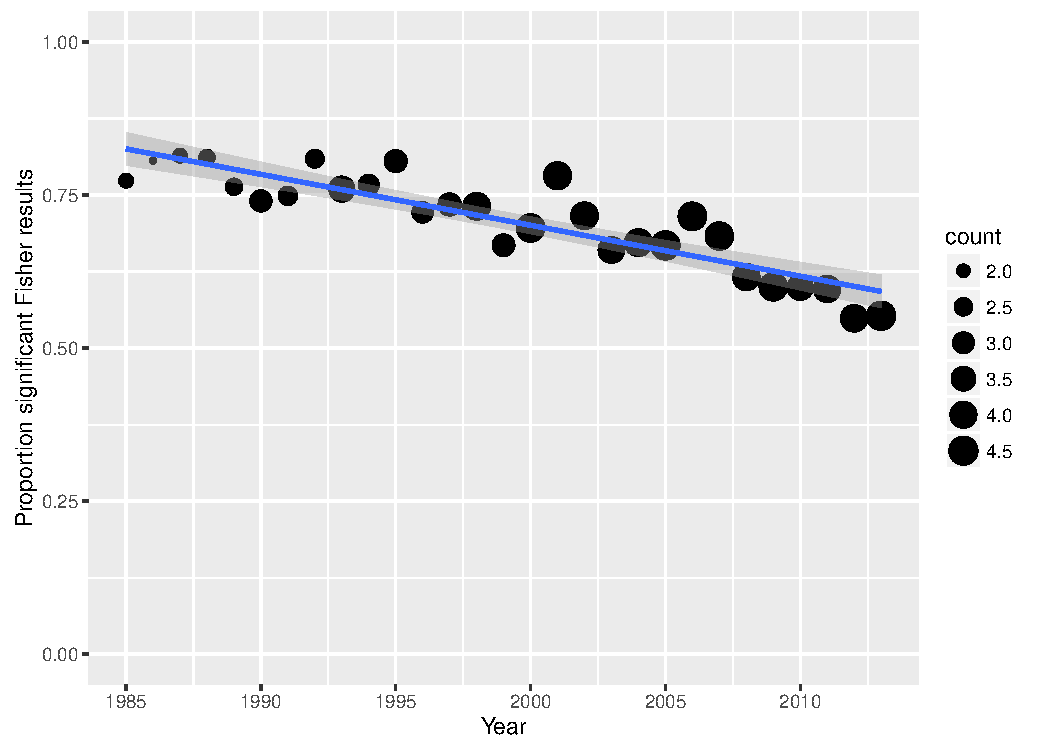
\includegraphics{../figures/Fig4.pdf}
\end{center}
\caption{Proportion of papers reporting nonsignificant results in a given year, showing evidence for false negative results. Larger point size indicates a higher mean number of nonsignificant results reported in that year.}
\label{fig:fig4}
\end{figure}

\begin{figure}
\begin{center}
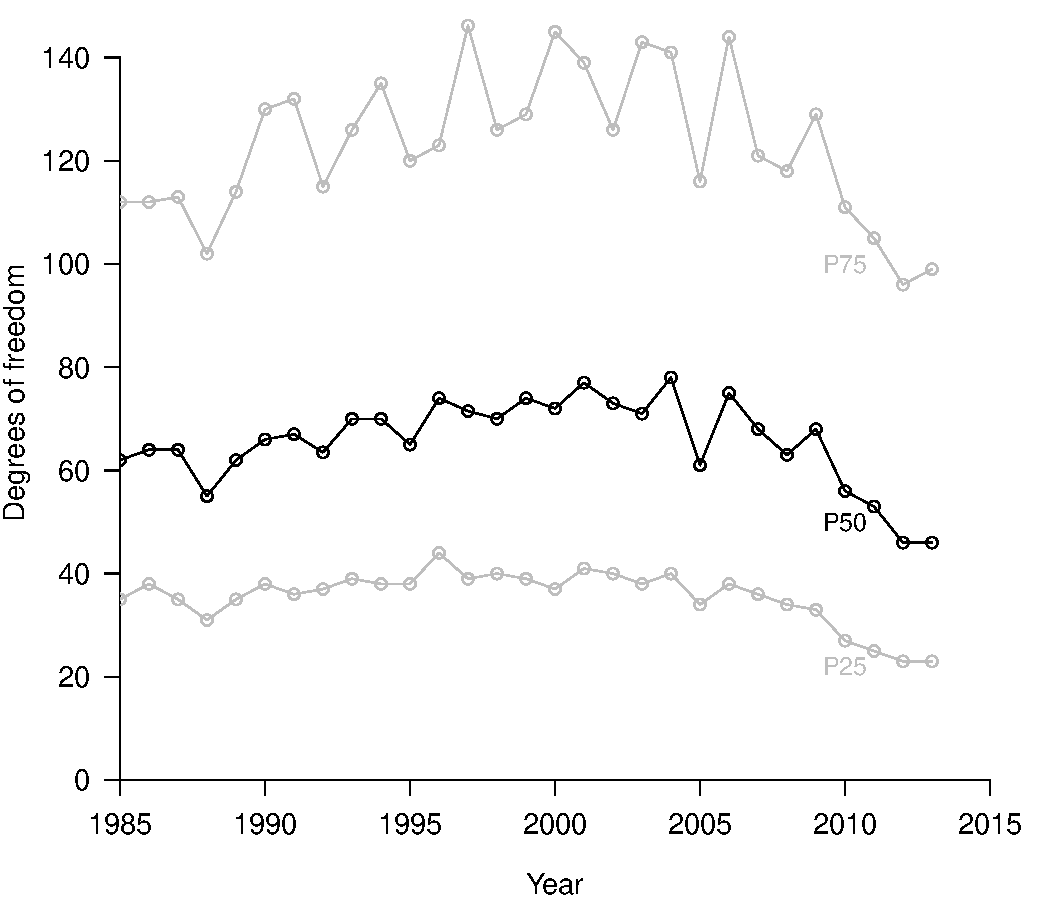
\includegraphics{../figures/Fig5.pdf}
\end{center}
\caption{Sample size development in psychology throughout 1985-2013, based on degrees of freedom across 258,050 test results. P25 = 25th percentile. P50 = 50th percentile (i.e., median). P75 = 75th percentile.}
\label{fig:fig5}
\end{figure}

\subsection*{Discussion}

The result that 2 out of 3 papers containing nonsignificant results show evidence of at least one false negative empirically verifies previously voiced concerns about insufficient attention for false negatives \cite{Fiedler2012-gx}. The Fisher test proved a powerful test to inspect for false negatives in our simulation study, where three nonsignificant results already results in high power to detect evidence of a false negative if sample size is at least 33 per result and the population effect is medium. Journals differed in the proportion of papers that showed evidence of false negatives, but this was largely due to differences in the amount of nonsignificant results reported. More generally, we observed that more nonsignificant results were reported in 2013 than in 1985. 

The repeated concern about power and false negatives throughout the last decades seems not to have trickled down into substantial change in psychology research practice. Cohen \cite{Cohen1962-jc} and Sedlmeier and Gigerenzer \cite{Sedlmeier1989-yc} already voiced concern decades ago and showed that power in psychology was low. Fiedler et al. \cite{Fiedler2012-gx} contended that false negatives are harder to detect in the current scientific system and therefore warrant more concern. Despite recommendations of increasing power by increasing sample size, we found no evidence for increased sample size (see Figure \ref{fig:fig5}). To the contrary, the data indicate that sample sizes have been remarkably stable since 1985, despite the improved ease of collecting participants with data collection tools such as online services.

However, what has changed is the amount of nonsignificant results reported in the literature. Our data show that more nonsignificant results are reported throughout the years (see Figure \ref{fig:fig2}), which seems contrary to findings that indicate that relatively more significant results are being reported \cite{Fanelli2011-xa, Sterling1995-fe, Sterling1959-pf,De_Winter2015-ru}. It would seem the field is not shying away from publishing negative results per se, as proposed before \cite{Fanelli2011-xa,Greenwald1975-ck,Nosek2012-aw,Rosenthal1979-lx,Schimmack2012-du}, but whether this is also the case for results relating to hypotheses of explicit interest in a study and not all results reported in a paper, requires further research. Other research strongly suggests that most reported results relating to hypotheses of explicit interest are statistically significant \cite{Open_Science_Collaboration2015-zs}.

\section*{Application 2: Evidence of false negative gender effects in eight major psychology journals}

In order to illustrate the practical value of the Fisher test to test for evidential value of (non)significant $p$-values, we investigated gender related effects in a random subsample of our database. Gender effects are particularly interesting because gender is typically a control variable and not the primary focus of studies. Hence, we expect little $p$-hacking and substantial evidence of false negatives in reported gender effects in psychology. We apply the Fisher test to significant and nonsignificant gender results to test for evidential value \cite{Van_Assen2015-gg,Simonsohn2014-dm}. More precisely, we investigate whether evidential value depends on whether the result is statistically significant or not, and whether the results were in line with expectations expressed in the paper, or not.

\subsection*{Method}

We planned to test for evidential value in six categories (expectation [3 levels] $\times$ significance [2 levels]). Expectations were specified as '$H_1$ expected', '$H_0$ expected', or 'no expectation'. Prior to data collection, we assessed the required sample size for the Fisher test based on research on the gender similarities hypothesis \cite{Hyde2005-gj}. We calculated that the required number of statistical results for the Fisher test, given $r=.11$ \cite{Hyde2005-gj} and 80\% power, is 15 $p$-values per condition, requiring 90 results in total. However, the six categories are unlikely to occur equally throughout the literature, hence we sampled 90 significant and 90 nonsignificant results pertaining to gender, with an expected cell size of 30 if results are equally distributed across the six cells of our design. Significance was coded based on the reported $p$-value, where $\leq.05$ was used as the decision criterion to determine significance \cite{Nuijten2015-od}.

We sampled the 180 gender results from our database of over 250,000 test results in four steps. First, we automatically searched for "gender", "sex", "female" AND "male", " man" AND " woman" [sic], or " men" AND " women" [sic] in the $100$ characters before the statistical result and $100$ after the statistical result (i.e., range of $200$ characters surrounding the result), which yielded 27,523 results. Second, the first author inspected $500$ characters before and after the first result of a randomly ordered list of all 27,523 results and coded whether it indeed pertained to gender. This was done until 180 results pertaining to gender were retrieved from 180 different articles. Third, these results were independently coded by all authors with respect to the expectations of the original researcher(s) (coding scheme available at \url{osf.io/9ev63}). The coding included checks for qualifiers pertaining to the expectation of the statistical result (confirmed/theorized/hypothesized/expected/etc.). If researchers reported such a qualifier, we assumed they correctly represented these expectations with respect to the statistical significance of the result. For example, if the text stated "as expected no evidence for an effect was found, $t(12)=1, p=.337$" we assumed the authors expected a nonsignificant result. Fourth, discrepant codings were resolved by discussion (25 cases [13.9\%]; two cases remained unresolved and were dropped). 178 valid results remained for analysis.

Prior to analyzing these 178 $p$-values for evidential value with the Fisher test, we transformed them to variables ranging from 0 to 1. Statistically nonsignificant results were transformed with Equation \ref{pistar}; statistically significant $p$-values were divided by alpha (.05; \cite{Van_Assen2015-gg,Simonsohn2014-dm}).

\subsection*{Results}


The coding of the 178 results indicated that results rarely specify whether these are in line with the hypothesized effect (see Table \ref{tab:tab5}). For the 178 results, only 15 clearly stated whether their results were as expected, whereas the remaining 163 did not. Illustrative of the lack of clarity in expectations is the following quote: "\textit{As predicted, there was little gender difference [...] p < .06.}" As a result, the conditions significant-$H_0$ expected, nonsignificant-$H_0$ expected, and nonsignificant-$H_1$ expected contained too few results for meaningful investigation of evidential value (i.e., with sufficient statistical power).

\begin{table}[htbp]
\caption{Number of gender results coded per condition in a 2 (significance: significant or nonsignificant) by 3 (expectation: $H_0$ expected, $H_1$ expected, or no expectation) design. Cells printed in bold had sufficient results to inspect for evidential value.}
\rowcolors{2}{gray!25}{white}
% \begin{adjustbox}{width=\textwidth,totalheight=\textheight,keepaspectratio,angle=0}
\centering
\begin{tabular}{lrrr}
& $H_0$ expected & $H_1$ expected & No expectation \\
\hline
Significant    & 0           & \textbf{12}          & \textbf{76}             \\
Nonsignificant & 2           & 1           & \textbf{87}     \\
\hline
\end{tabular}
% \end{adjustbox}
\label{tab:tab5}
\end{table}

\begin{figure}
\begin{center}
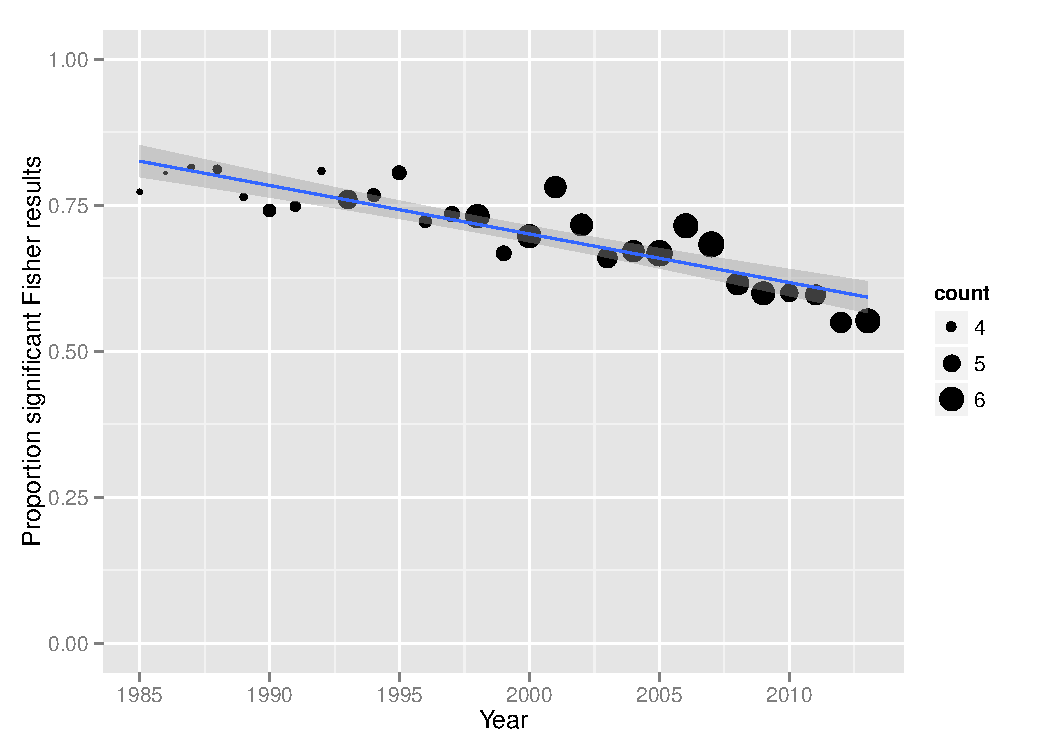
\includegraphics{../figures/Fig6.pdf}
\end{center}
\caption{Probability density distributions of the $p$-values for gender effects, split for nonsignificant and significant results. A uniform density distribution indicates the absence of a true effect.}
\label{fig:fig6}
\end{figure}

% these results are available in the code chunk above
Figure \ref{fig:fig6} presents the distributions of both transformed significant and non-significant $p$-values. For significant results, applying the Fisher test to the $p$-values showed evidential value for a gender effect both when an effect was expected ($\chi^2(24)=358.725$, $p<.001$) and when no expectation was presented at all ($\chi^2(152)=1093.884$, $p<.001$). Similarly, applying the Fisher test to nonsignificant gender results without stated expectation yielded evidence of at least one false negative ($\chi^2(174)=324.374$, $p<.001$). Unfortunately, we could not examine whether evidential value of gender effects is dependent on the hypothesis/expectation of the researcher, because these effects are most frequently reported without stated expectations. 

\subsection*{Discussion}

We observed evidential value of gender effects both in the statistically significant (no expectation or $H_1$ expected) and nonsignificant results (no expectation). The data from the 178 results we investigated indicated that in only 15 cases the expectation of the test result was clearly explicated. This indicates that based on test results alone, it is very difficult to differentiate between results that relate to a priori hypotheses and results that are of an exploratory nature. The importance of being able to differentiate between confirmatory and exploratory results has been previously demonstrated \cite{Wagenmakers2012-jq} and has been incorporated into the Transparency and Openness Promotion guidelines (TOP; \cite{Nosek2015-nr}) with explicit attention paid to pre-registration.

\section*{Application 3: Reproducibility Project Psychology}

Out of the 100 replicated studies in the RPP, 64 did not yield a statistically significant effect size, despite the fact that high replication power was one of the aims of the project \cite{Open_Science_Collaboration2015-zs}. Regardless, the authors suggest "\textit{… that at least one replication could be a false negative}" (p. aac4716-4). Here we estimate how many of these nonsignificant replications might be false negative, by applying the Fisher test to these nonsignificant effects.

\subsection*{Method}

Of the 64 nonsignificant studies in the RPP data (\url{osf.io/fgjvw}), we selected the 63 nonsignificant studies with a test statistic. We eliminated one result because it was a regression coefficient that could not be used in the following procedure. We first applied the Fisher test to the nonsignificant results, after transforming them to variables ranging from 0 to 1 using equations \ref{pistar} and \ref{fishertest}. Denote the value of this Fisher test by $Y$; note that under the $H_0$ of no evidential value $Y$ is $\chi^2$-distributed with 126 degrees of freedom.

Subsequently, we hypothesized that $X$ out of these 63 nonsignificant results had a weak, medium, or strong population effect size (i.e., $\rho=.1$, $.3$, $.5$, respectively; \cite{Cohen1988-wg}) and the remaining $63-X$ had a zero population effect size. For each of these hypotheses, we generated 10,000 data sets (see next paragraph for details) and used them to approximate the distribution of the Fisher test statistic (i.e., $Y$). Using this distribution, we computed the probability that a $\chi^2$-value exceeds $Y$, further denoted by $p_Y$. We then used the inversion method \cite{Casella2002-cy} to compute confidence intervals of $X$, the number of nonzero effects. Specifically, the confidence interval for $X$ is ($X_{LB};X_{UB}$), where $X_{LB}$ is the value of $X$ for which $p_Y$ is closest to $.025$ and $X_{UB}$ is the value of $X$ for which $p_Y$ is closest to $.975$. We computed three confidence intervals of $X$: one for the number of weak, medium, and large effects.

We computed $p_Y$ for a combination of a value of $X$ and a true effect size using 10,000 randomly generated datasets, in three steps. For each dataset we: 
\begin{enumerate}
\item Randomly selected $X$ out of 63 effects which are supposed to be generated by true nonzero effects, with the remaining $63-X$ supposed to be generated by true zero effects;
\item Given the degrees of freedom of the effects, we randomly generated $p$-values under the $H_0$ using the central distributions and non-central distributions (for the $63-X$ and $X$ effects selected in step 1, respectively);
\item The Fisher statistic $Y$ was computed by applying Equation \ref{fishertest} to the transformed $p$-values (see Equation \ref{pistar}) of step 2. 
\end{enumerate}
Probability $p_Y$ equals the proportion of 10,000 datasets with $Y$ exceeding the value of the Fisher statistic applied to the RPP data. See \url{osf.io/egnh9} for the analysis script to compute the confidence intervals of $X$. 

\subsection*{Results}



Upon reanalysis of the 63 statistically nonsignificant replications within RPP we determined that many of these "failed" replications say hardly anything about whether there are truly no effects. The Fisher test of these 63 nonsignificant results indicated some evidence for the presence of at least one false negative finding ($\chi^2(126)=155.2382$, $p=0.039$). Assuming $X$ small nonzero true effects among the nonsignificant results yields a confidence interval of 0-63 (0-100\%). More specifically, if all results are in fact true negatives then $p_Y=.039$, whereas if all true effects are $\rho=.1$ then $p_Y=.872$. Hence, the 63 statistically nonsignificant results of the RPP are in line with any number of true small effects --- from none to all. Consequently, we cannot draw firm conclusions about the state of the field psychology concerning the frequency of false negatives using the RPP results and the Fisher test, when all true effects are small. Assuming $X$ medium or strong true effects underlying the nonsignificant results from RPP yields confidence intervals 0-21 (0-33.3\%) and 0-13 (0-20.6\%), respectively. In other words, the 63 statistically nonsignificant RPP results are also in line with some true effects actually being medium or even large.

\subsection*{Discussion}

The reanalysis of the nonsignificant RPP results using the Fisher method demonstrates that any conclusions on the validity of individual effects based on "failed" replications, as determined by statistical significance, is unwarranted and irresponsible. This was also noted by both the original RPP team \cite{Open_Science_Collaboration2015-zs,Anderson2016-bv} and in a critique of the RPP \cite{Gilbert2016-mi}. Replication efforts such as the RPP or the Many Labs project remove publication bias and result in a less biased assessment of the true effect size. Nonetheless, single replications should not be seen as the definitive result, considering that these results indicate there remains much uncertainty about whether a nonsignificant result is a true negative or a false negative. The explanation of this finding is that most of the RPP replications, although often statistically more powerful than the original studies, still did not have enough statistical power to distinguish a true small effect from a true zero effect \cite{Maxwell2015-yb}. Interpreting results of replications should therefore also take the precision of the estimate of both the original and replication into account \cite{Cumming2014-fi}.

\section*{General discussion}

Much attention has been paid to false positive results in recent years. Our study demonstrates the importance of focusing on false negatives as well. We examined evidence for false negatives in nonsignificant results in three different ways. To this end, we adapted the Fisher method to detect the presence of at least one false negative in a set of statistically nonsignificant results; simulations indicated it to be a powerful method for that purpose. The three applications indicated that (i) approximately two out of three psychology articles reporting nonsignificant results contain evidence for at least one false negative, (ii) nonsignificant results on gender effects contain evidence of true nonzero effects, and (iii) the statistically nonsignificant replications from the Reproducibility Project Psychology (RPP) do not warrant conclusions about the absence or presence of true zero effects underlying these nonsignificant results (RPP does yield less biased estimates of the effect; the original studies severely overestimated the effects of interest).

The methods used in the three different applications provide crucial context to interpret the results. In applications 1 and 2, we did not differentiate between main and peripheral results. Hence, the interpretation of a significant Fisher test result pertains to the evidence of at least one false negative in all reported results, not the evidence for at least one false negative in the main results. Nonetheless, even when we focused only on the main results in application 3, the Fisher test does not indicate specifically which result is false negative, only whether there is evidence for a false negative in a set of results. As such, the Fisher test is primarily useful to test a set of potentially underpowered results in a more powerful manner, albeit that the result then applies to the complete set. Additionally, in applications 1 and 2 we focused on results reported in eight psychology journals; extrapolating the results to other journals might not be warranted given that there might be substantial differences in the type of results reported in other journals or fields. 

More generally, our results in these three applications confirm that the problem of false negatives in psychology remains pervasive. Previous concern about power \cite{Cohen1962-jc,Sedlmeier1989-yc,Bakker2012-tf,Marszalek2011-rf}, which was even addressed by an APA Statistical Task Force in 1999 that recommended increased statistical power \cite{Wilkinson_APA_Task_Force_on_Statistical_Inference1999-ht}, seems not to have resulted in actual change \cite{Marszalek2011-rf}. A potential explanation for this lack of change is that researchers overestimate statistical power when designing a study for small effects \cite{Bakker2016-nj}.

Reducing the emphasis on binary decisions in individual studies and increasing the emphasis on the precision of a study might help reduce the problem of decision errors. For example, a large but statistically nonsignificant study might yield a confidence interval (CI) of the effect size of [-0.01; 0.05], whereas a small but significant study might yield a CI of [0.01; 1.30]. In a purely binary decision mode, the small but significant study would result in the conclusion that there is an effect because it provided a statistically significant result, despite it containing much more uncertainty than the larger study about the underlying true effect size. In a precision mode, the large study provides a more certain estimate and therefore is deemed more informative and provides the best estimate. Using meta-analyses to combine estimates obtained in studies on the same effect may further increase the overall estimate’s precision. Although the emphasis on precision and the meta-analytic approach is fruitful in theory, we should realize that publication bias will result in precise but biased (overestimated) effect size estimates of meta-analyses \cite{Nuijten2015-kh}.

\subsection*{Limitations and further research}

For all three applications, the Fisher tests' conclusions are limited to detecting at least one false negative in a \textit{set of results}. The method cannot be used to draw inferences on individuals results in the set. To draw inferences on the true effect size underlying one specific observed effect size, generally more information (i.e., studies) is needed to increase the precision of the effect size estimate.

Another potential caveat relates to the data collected with the \texttt{R} package \texttt{statcheck} and used in applications 1 and 2. \texttt{statcheck} extracts inline, APA style reported test statistics, but does not include results included from tables or results that are not reported as the APA prescribes. Consequently, our results and conclusions may not be generalizable to \textit{all} results reported in articles. 

Given that the results indicate that false negatives are still a problem in psychology, albeit slowly on the decline in published research, further research is warranted. Further research could focus on comparing evidence for false negatives in main and peripheral results. Our results in combination with results of previous studies suggest that publication bias mainly operates on results of tests of main hypotheses, and less so on peripheral results. Another venue for future research is using the Fisher test to re-examine evidence in the literature on certain other effects or often-used covariates, such as age and race, or to see if it helps researchers prevent dichotomous thinking with individual $p$-values \cite{Hoekstra2006}. Finally, the Fisher test may and is also used to meta-analyze effect sizes of different studies. Whereas Fisher used his method to test the null-hypothesis of an underlying true zero effect using several studies’ $p$-values, the method has recently been extended to yield unbiased effect estimates using only statistically significant $p$-values. The principle of uniformly distributed $p$-values given the true effect size on which the Fisher method is based, also underlies newly developed methods of meta-analysis that adjust for publication bias, such as $p$-uniform \cite{Van_Assen2015-gg} and $p$-curve \cite{Simonsohn2014-dm}. Extensions of these methods to include nonsignificant as well as significant $p$-values and to estimate heterogeneity are still under construction.

To conclude, the three applications that were presented indicate that false negatives remain a problem in the psychology literature, despite the decreased attention and that we should be wary to interpret statistically nonsignificant results as there being no effect in reality. One way to combat this interpretation of statistically nonsignificant results is to incorporate testing for potential false negatives, which the Fisher method facilitates in a highly approachable manner  (a spreadsheet for carrying out such a test is available at \url{https://osf.io/tk57v/}).

%%%%%%%%%%%%%%%%%%%%%%%%%%%
\section*{Appendix A}
\label{apA}
\subsection*{Examining statistical properties of the Fisher test}
The Fisher test to detect false negatives is only useful if it is powerful enough to detect evidence of at least one false negative result in papers with few nonsignificant results. Therefore we examined the specificity and sensitivity of the Fisher test to test for false negatives, with a simulation study of the one sample $t$-test. Throughout this paper, we apply the Fisher test with $\alpha_{Fisher}=0.10$, because tests that inspect whether results are "too good to be true" typically also use alpha levels of 10\% \cite{Sterne2000-wh,Ioannidis2007-hh,Francis2012-kw}. The simulation procedure was carried out for conditions in a three-factor design, where power of the Fisher test was simulated as a function of sample size $N$, effect size $\eta$, and $k$ test results. The three factor design was a 3 (sample size $N$: 33, 62, 119) by 100 (effect size $\eta$: .00, .01, .02, ..., .99) by 18 ($k$ test results: 1, 2, 3, ..., 10, 15, 20, ..., 50) design, resulting in 5,400 conditions. The levels for sample size were determined based on the 25th, 50th, and 75th percentile for the degrees of freedom ($df2$) in the observed dataset for Application 1. Each condition contained 10,000 simulations. The power of the Fisher test for one condition was calculated as the proportion of significant Fisher test results given $\alpha_{Fisher}=0.10$. If the power for a specific effect size $\eta$ was $\geq99.5\%$, power for larger effect sizes were set to 1.

We simulated false negative $p$-values according to the following six steps (see Figure \ref{fig:appendixa}). First, we determined the critical value under the null distribution. Second, we determined the alternative distribution by computing the non-centrality parameter ($\delta=(\eta^2/1-\eta^2)N$; \cite{Steiger1997-qq,Smithson2001-aw}). Third, we calculated the probability that a result under the alternative distribution was, in fact, nonsignificant (i.e., $\beta$). Fourth, we randomly sampled, uniformly, a value between $0-\beta$. Fifth, with this value we determined the accompanying $t$-value. Finally, we computed the $p$-value for this $t$-value under the null distribution. 

\begin{figure}[!ht]
\centering
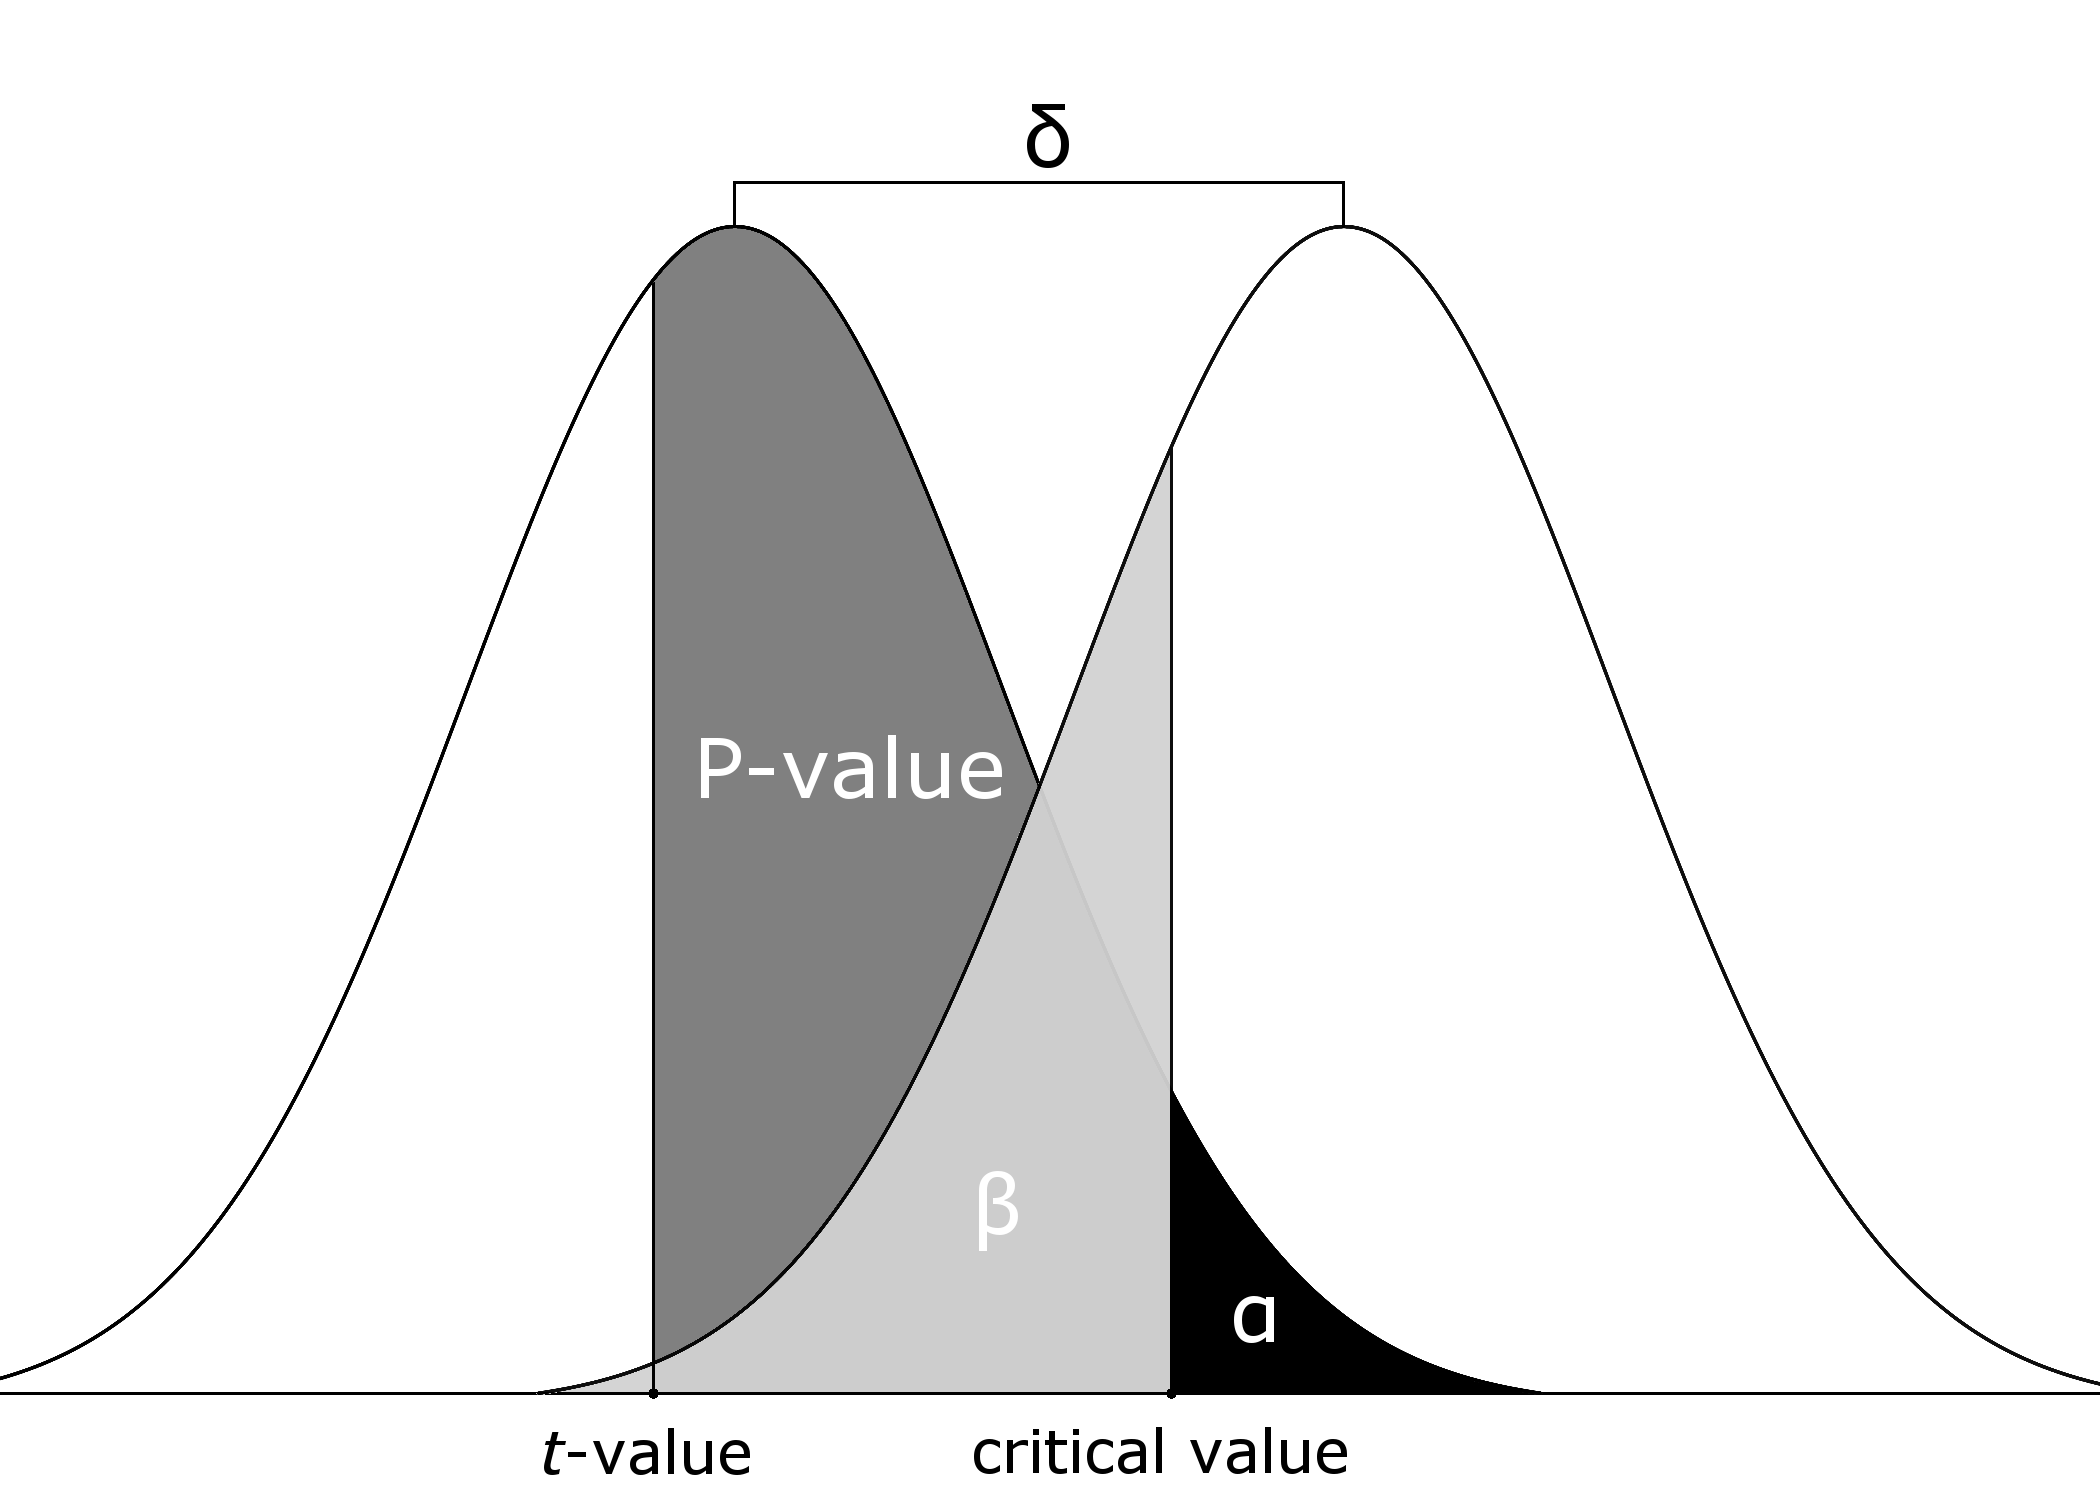
\includegraphics[width=0.75\textwidth]{../figures/appendix_a}
\caption{Visual aid for simulating one nonsignificant test result. The critical value from $H_0$ (left distribution) was used to determine $\beta$ under $H_1$ (right distribution). A value between 0 and $\beta$ was drawn, $t$-value computed, and $p$-value under $H_0$ determined.}
\label{fig:appendixa}
\end{figure}

We repeated the procedure to simulate a false negative $p$-value $k$ times and used the resulting $p$-values to compute the Fisher test. Before computing the Fisher test statistic, the nonsignificant $p$-values were transformed (see Equation \ref{pistar}). Subsequently, we computed the Fisher test statistic and the accompanying $p$-value according to Equation \ref{fishertest}. 

\section*{Appendix B}
\label{apB}
\subsection*{Effect computation}

The $t$, $F$, and $r$-values were all transformed into the effect size $\eta^2$, which is the explained variance for that test result and ranges between 0 and 1, for comparing observed to expected effect size distributions. For $r$-values, this only requires taking the square (i.e., $r^2$). $F$ and $t$-values were converted to effect sizes by
\begin{equation}
\eta^2=\frac{\frac{F\times df_1}{df_2}}{\frac{F\times df_1}{df_2}+1}
\label{eq:b1}
\end{equation}
where $F=t^2$ and $df_1=1$ for $t$-values. Adjusted effect sizes, which correct for positive bias due to sample size, were computed as
\begin{equation}
\eta^2_{adj}=\frac{\frac{F\times df_1}{df_2}-\frac{df_1}{df_2}}{\frac{F\times df_1}{df_2}+1}
\label{eq:b2}
\end{equation}
which shows that when $F=1$ the adjusted effect size is zero. For $r$-values the adjusted effect sizes were computed as \cite{Ivarsson2013-rm}
\begin{equation}
\eta^2_{adj}=\eta^2-([1-\eta^2]\times\frac{v}{N-v-1})
\label{eq:b3}
\end{equation}
where $v$ is the number of predictors. It was assumed that reported correlations concern simple bivariate correlations and concern only one predictor (i.e., $v=1$). This reduces the previous formula to
\begin{equation}
\eta^2_{adj}=\eta^2-\frac{1-\eta^2}{df}
\label{eq:b4}
\end{equation}
where $df=N-2$.
\bibliography{../bibliography/library}
\end{document}
